Although \app{} supports identification and testing of GEF components
out-of-the-box, it is highly recommended that application developers enhance
this support by implementing an accessibility plug-in for their application. Such a
plug-in makes identification of GEF components more robust and allows \app{}
tests to reference additional components, such as connection anchors.

Apart from the general description for creating toolkit extensions in the
extension manual, we give further information for extending the GEF toolkit. The
following sections explain how to develop a GEF accessibility plug-in.

\section{Creating an accessibility plug-in}

\subsection{Setting up your Workspace}
Although you can use the IDE of your choice to develop your accessibility
plug-in, this guide will use Eclipse with PDE plug-ins.

\begin{enumerate}
\item Once you have created your new workspace, change that workspace's
\textbf{Target Platform} by using the description mentioned in the extension
manual, as well as all plug-ins that make up your \gdaut{}.

\item Create a new \textbf{Plug-in Project}. The default values proposed by the
wizard are acceptable, so simply enter a name for your new accessibility project
and complete the wizard without additional modifications.

\item You now have a workspace with a properly configured target platform as
well as a new plug-in project. You can now begin developing your GEF
toolkit extension.
\end{enumerate}

\subsection{Walkthrough}
The first step for implementing your accessibility plug-in is to create
identifiers for each type of GEF component that you wish to make accessible for
\app{} tests. An identifier is a Java class that implements
\bxshell{IEditPartIdentifier} from the package named
\bxname{org.eclipse.jubula.rc.rcp.e3.gef.identifier} and provides \app{} with
additional and/or more precise information about a specific \bxshell{EditPart}
from the package named \bxname{org.eclipse.gef}. The granularity of your
identifier classes will depend on the class hierarchy of the edit parts in the
\gdaut{}. For example, if many of the edit parts share a common superclass, then
you can write a single Identifier for that superclass that will be able to
provide accessibility for all edit parts that inherit from that superclass. See
the example in section \ref{gefreference}, which shows a sample implementation.

The next step is to create an adapter factory. This extension will provide
\app{} with information regarding which identifier to use for each edit part.
\begin{enumerate}
\item  Open the \bxshell{plugin.xml} file from your accessibility plug-in and
select the \textbf{Extension} tab. % (\bxfigref{extensionstab}).

% \begin{figure}[h]
% \begin{center}
% 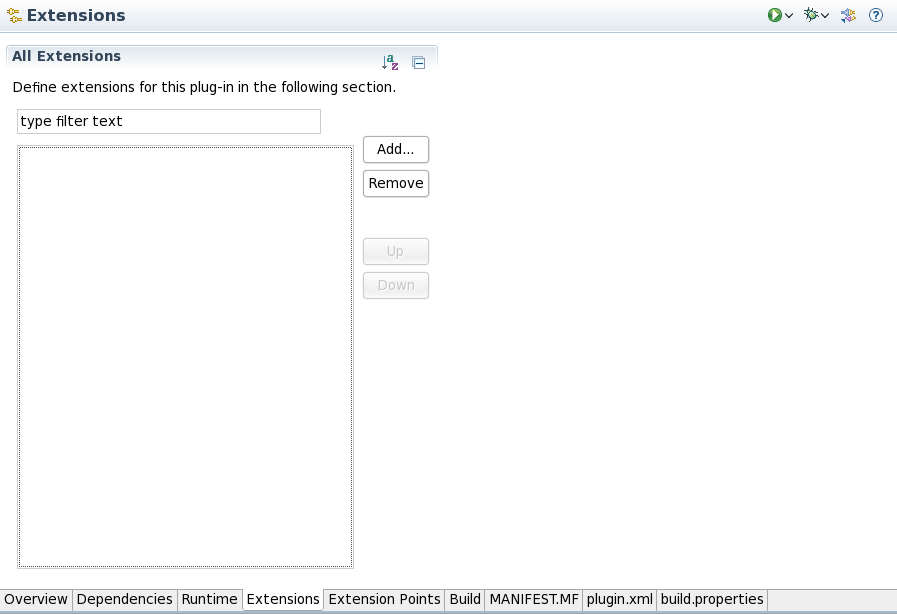
\includegraphics[width=12.5cm]{gefextension/PS/extensionstab}
% \caption{Plug-in Editor with Extensions tab selected}
% \label{extensionstab}
% \end{center}
% \end{figure}

\item Add an instance of the \bxname{org.eclipse.core.runtime.adapters}
extension.
\item Add a \textbf{factory} to the new extension for each type of GEF component
for which you wish to provide accessibility. Each factory must implement
\bxshell{IEditPartIdentifier} from the package named
\bxname{org.eclipse.jubula.rc.rcp.e3.gef.identifier} to provide adapters from
the GEF component that implements \bxshell{EditPart} from
\bxname{org.eclipse.gef}. % (\bxfigref{factory}).

% \begin{figure}[h]
% \begin{center}
% 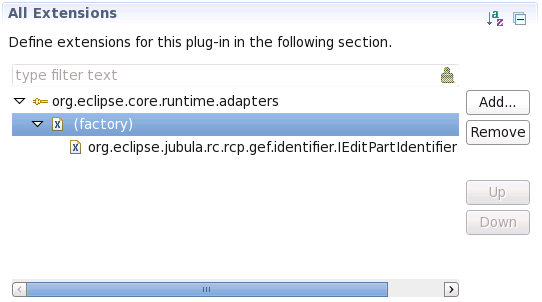
\includegraphics[width=12.5cm]{gefextension/PS/factory}
% \caption{Plug-in Editor with defined Adapter Factory}
% \label{factory}
% \end{center}
% \end{figure}

\item Once you have defined your adapter factory, you will need to implement it.
Your adapter factory, which must implement \bxshell{IAdapaterFactory} from the
package named \bxname{org.eclipse.core.runtime}, provides appropriate
instances of your created identifiers for a given edit part. See
\bxpref{gefreference} for a sample implementation.


\item Once you have created your identifiers and adapter factories, you can
export and deploy your plug-in to use it in your \gdaut{}.
%(\bxfigref{exportplugin}).

\bxtipp{When starting your \gdaut{} after adding or replacing your accessibility
plug-in, it is recommended that the \gdaut{} starts with the \bxshell{-clean}
parameter.}

% \begin{figure}[h]
% \begin{center}
% 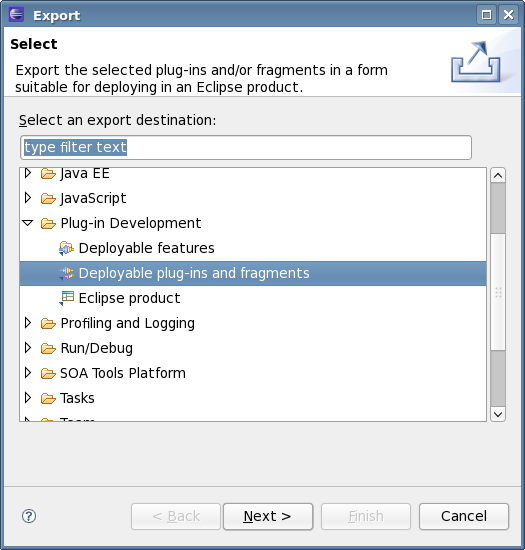
\includegraphics[width=12.5cm]{gefextension/PS/exportplugin}
% \caption{Exporting the Project to a Plug-in}
% \label{exportplugin}
% \end{center}
% \end{figure}

\end{enumerate}

\section{Accessibility plug-in example}
\label{gefreference}
A sample accessibility plug-in for certain elements of the Logic Diagram sample
plug-in project (contributed from the GEF plug-ins to Eclipse's New Project
Wizard) are included in the installation of \app{}. A default implementation can
be found in the directory \bxshell{examples/development/gef}. There you will
find a zip-file containing a full accessibility plug-in example.

You can import the sample accessibility plug-in into an Eclipse workspace in
order to examine the general structure. %(\bxfigref{newlogicwizard}).
The Java documentation of the source code, which is included in the target
platform definition, contains information about \bxshell{IEditPartIdentifier}
from the package named\\
\bxname{org.eclipse.jubula.rc.rcp.gef.identifier}.


% \begin{figure}[h]
% \begin{center}
% 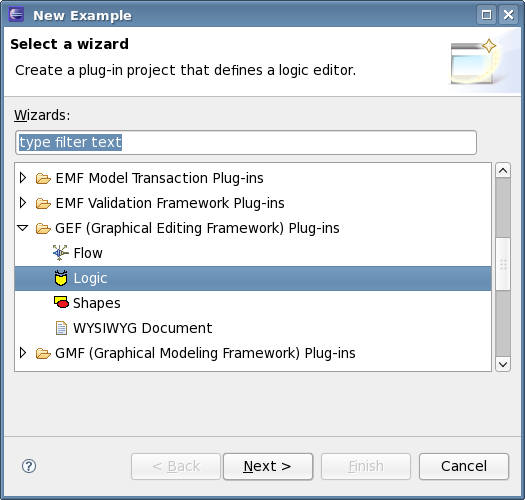
\includegraphics[width=12.5cm]{gefextension/PS/newlogicwizard}
% \caption{Creating the 'Logic' Project}
% \label{newlogicwizard}
% \end{center}
% \end{figure}
